\section{HRRadarPose}
Inspired by HRNet~\cite{hrnet}, renowned for its adeptness in extracting high-resolution representations, we build an architecture, HRRadarPose, with fully 3D convolutional layers.
By treating the Doppler axis, \(D\), as the input channels, our model extracts volumetric spatial features along the \(Z\), \(Y\), and \(X\) axes, representing vertical, horizontal, and depth directions in the Cartesian coordinate system. 
The HRRadarPose architecture is designed to preserve spatial resolution and assimilate semantic information from the 4D radar tensors, maintaining high-resolution representations and enabling the exchange of information between features of different resolutions during stage transitions.
Figure~\ref{fig:radarpose} illustrates an instance of the HRRadarPose structure with three stages. 
The structure starts with using 3D convolutional layers to transform the 4D radar tensors, \(T \in \mathbb{R}^{D \times Z \times Y \times X}\), into features, \(f_{in} \in \mathbb{R}^{C_{1} \times Z_{1} \times Y_{1} \times X_{1}}\). 
As the network proceeds from one stage to the next, it develops additional branches through strided convolution to widen the receptive field. 
Each branch \(i\) employs strided convolution to elevate its input feature \(f_{i}\) to a feature \(f_{i+1}\) in the succeeding branch \(i+1\), simultaneously doubling the channels and halving the spatial dimensions, \(f_{i+1} \in \mathbb{R}^{ 2C_{i} \times \frac{Z_{i}}{2} \times \frac{Y_{i}}{2} \times \frac{X_{i}}{2} }\).
Within each stage, a series of \(P\) modules execute \(M\) parallel convolutions. 
To align feature dimensions from different branches for information exchange, we use strided convolution followed by upsampling. 
At the end of the backbone, we take the feature with the highest resolution to serve as a unified representation for the pose estimation head. 
In the pose estimation head, two 3D convolutional branches are employed to process these features further. 
This bifurcation generates two outputs: a distribution map signifying the confidence of locating the human center and the location offset of joint keypoints. 
The right part of Figure~\ref{fig:radarpose} shows the decoding of the HRRadarPose network's output to multi-person poses.
The process starts with picking top-$k$ human centers, \(C_S\), with confidence scores over a threshold value. 
We denote these picked centers' indices as \(S\).
Then, we query the centers corresponding joint keypoints' offsets, \(K_S\), by looking up the output map of keypoint offsets head at \(S\). 
Lastly, we decode their joint keypoint locations, \(J_S\), by summing \(K_S\) and \(C_S\). 
In scenarios with multiple people, we apply range non-maximum suppression (NMS) to reduce overlapping detections. Our method is favorable in two folds:
The HRRadarPose's architecture gains efficiency through a single-stage workflow, avoiding complexity brought by region-proposal-based methods ~\cite{zhao2018rf}. In addition, our pose estimation head inherently learns per person's joint keypoints refraining from ambiguity of association between people's identity and joints. 

\begin{figure}[t]
\centering
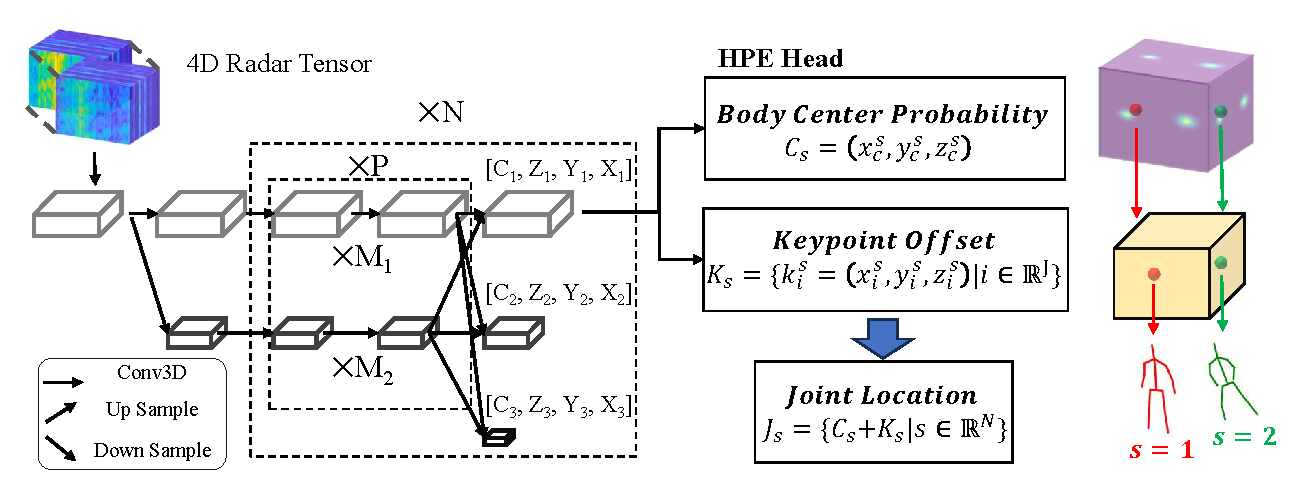
\includegraphics[width=1.0\linewidth]{fig/radarpose.pdf}
\caption{
 HRRadarPose's architecture consists of a 3D convolutional backbone and a pose estimation head, which generates a body center's confidence map and joint keypoint offsets map. 
 To infer multi-person poses, we decode the prediction by adding the picked bodies' centers with their corresponding keypoint offsets. 
}
\label{fig:radarpose}
\end{figure}


To train the center probability head, we use the pixel-wise focal loss as the classification loss, \( L_{class} \), defined as:
\begin{equation}
L_{class} =
\begin{cases}
    (1 - P_{xyz})^\alpha \log(P_{xyz}), & \text{if } Y_{xyz} = 1, \\
(1 - Y_{xyz})^\beta (P_{xyz})^\alpha \log(1 - P_{xyz}), & \text{otherwise},
\end{cases}
\end{equation} \ where \(Y_{xyz}\) is the three-dimensional human center Gaussian distribution map generated by pelvis locations, \(P_{xyz}\) is the probability of a person's presence at location, \((x,y,z)\), \(N\) is the number of foreground samples, \(\alpha\) and \(\beta\) are hyperparameters addressing class imbalance and focusing training on foreground samples.
To train the keypoint offset head, we construct the regression loss \(L_{reg}\) by taking the average of 15 keypoints' \(\mathcal{L}_{1}\), comparing the distance between predicted offsets and ground-truth offsets to the center location of a voxel in \(Y\) when \(Y_{xyz}\) equals to \(1\). 
The final loss is a weighted sum of \( L_{class} \) and \(L_{reg}\).
